\chapter{RESULTS}\label{result}

\textbf{Implementation}  We modified the published codes of the layer decomposition and MSERs, which are available on GitHub (https://github.com/ CraGL/Decompose-Single-Image-Into-Layers; https://github.com/idiap/mser) ,the differences between our algorithm and the available codes are explained in Section 4.2.1 and 5.2. Our algorithms were written in Python and vectorized using NumPy/SciPy. In our implementation, the parameters in Layer decomposition, ETF field, and MSERs are set the default values as in the original codes.\\ 
\textbf{Performance}  We performed the bas-relief generation on a variety Chinese paintings, and some Rosemaling paintings. We also performed our brush strokes extraction algorithm on some van Gogh's paintings, as described in Section \ref{comparevan}. All the paintings are from the internet.  All the tests were performed on a 6-core of 3.33 GHz Intel Core Xeon CPU with memory of 32 GB(RAM).\\
Table 3 further shows the running time of the proposed approach. Compared to the performance in \cite{tan2016decomposing} and \cite{nister2008linear}, there is no distinct difference. Additionally, the shape from shading algorithm does not consume much time since it depends on the segmented stroke regions. Our implementation is not multithreaded. \\
\textbf{Comparisons}  
As illustrated in section \ref{overview}, our method can be separated into three steps:layer decomposition, brush stroke extraction, bas-relief generation. We compared our work in each step with other alternative methods.\\
For layer decomposition, we compared the our algorithm with the Tan et al's work \cite{tan2016decomposing} in section \ref{comparelayer}, and we demonstrate our modified algorithm can better preserve the smoothness and completeness of brushstorkes in layers. \\
For stroke extraction, we compared our work with Li et al.'s work \cite{li2012rhythmic} in section \ref{comparevan}, and demonstrate that our method have a better performance in brush stroke extraction.\\
For bas-relief generation,we compared our work with Zeng et al.'s work \cite{zeng2014region} in section \ref{compare}, and we demonstrate our algorithm has better performance based on three factors mentioned in Section \ref{2dimagebased} : depth information, silhouettes and edges,fine details. \\
\textbf{Limitations}.\\ We discuss the limitations of this work as related to different steps in the method:
1) Layer decomposition: The paint colors based on building and simplify the  convex hull of input image in RGB space, sometimes, a paint color can be inside of the convex hull which can not be selected. With wrongly picked paint colors, the layer decomposition may not preserve or separate the brush strokes . 
2) Brush stroke extraction: some images can be too complex for proper segmentation, e.g., brush strokes highly blended with  multiple painting colors; hence, we cannot form meaningful regions and compute layering.

\begin{figure}[H]
	\centering
	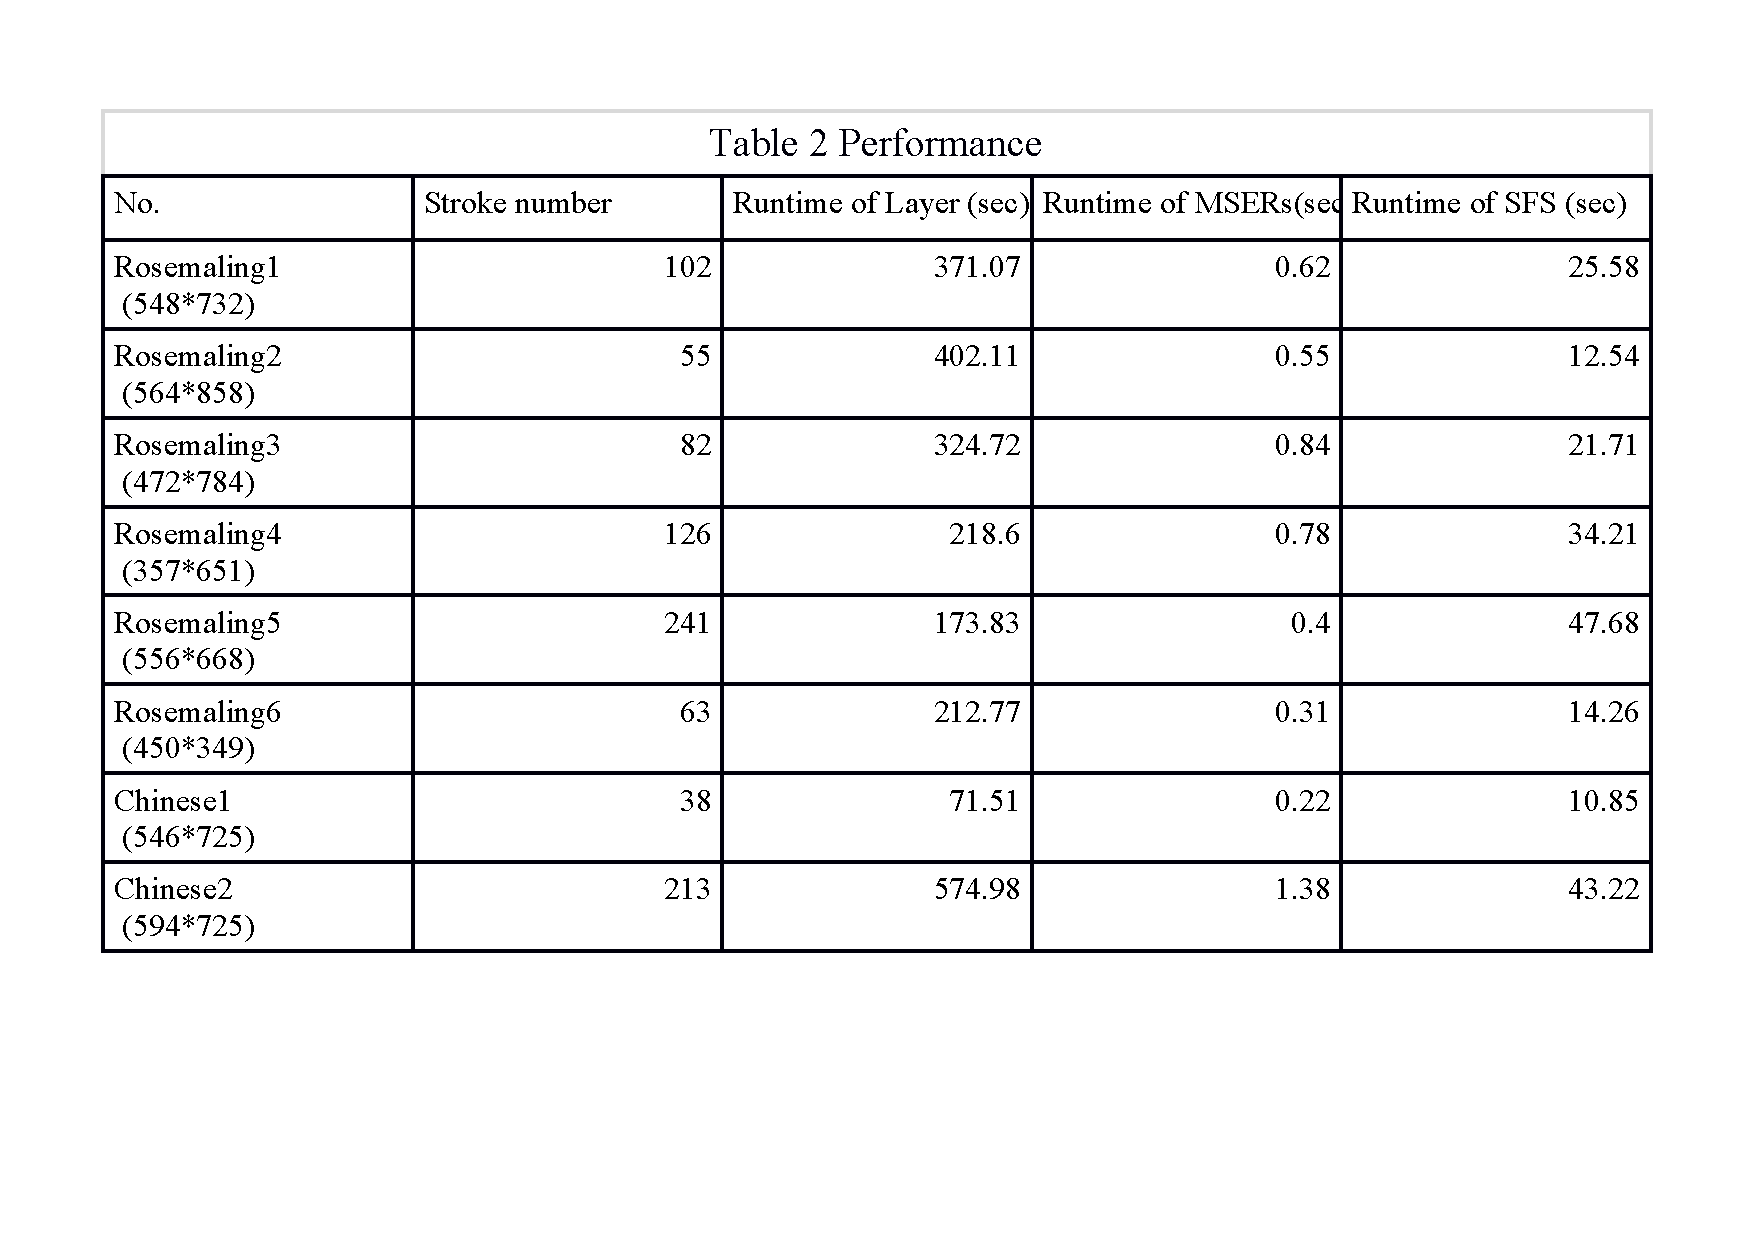
\includegraphics[width=14cm]{performance.pdf}

\end{figure}


